\chapter{Protótipo}\label{cap:proto}

		O projeto foi aplicado a um medidor de energia elétrica de dois terminais, conforme a Figura \ref{img:proto:meas}. Inicialmente projetado para medição de uma tensão e duas correntes em um sistema de quatro terminais, o bloco de amplificação e medição apresenta apenas uma tensão e uma corrente. A adição do circuito de medição de corrente extra pode ser realizada pela soldagem dos componentes necessários na placa.

		\begin{figure}[h!]
			\caption{Circuito de medição do protótipo}
			\label{img:proto:meas}
			\centering
			\begin{tikzpicture}[scale=1.0, 
								point/.style={circle, fill=black, ultra thin, inner sep=0.05cm},
								inout/.style={circle, draw, radius=4pt, thick}, 
								meter/.style={circle, draw, minimum size=1cm, align=center, thick}]
			\node (inneg) at (0,0)	[inout]	{};
			\node (inpos) at (0,4) [inout]	{};
			\node (ampneg) at (3,0) [meter] {A};
			\node (amppos) at (3,4) [meter] {A};
			\node (volt) at (5,2) [meter] {V};
			\node (ptneg) at (5,0) 	[point] {};
			\node (ptpos) at (5,4)	[point] {};
			\node (outneg) at (9,0)	[inout]	{};
			\node (outpos) at (9,4)[inout] {};
			\draw (inneg) node [text label, above] {Entrada\\(-)} -- (ampneg) -- (ptneg) -- (outneg) node [text label, above] {Saída\\(-)};
			\draw (inpos) node [text label, below] {Entrada\\(+)} -- (amppos) -- (ptpos) -- (outpos) node [text label, below] {Saída\\(+)};
			\draw (volt) -- (ptneg);
			\draw (volt) -- (ptpos);
			\draw (1,-1) 
				rectangle (7,5) 
				[dashed, draw=black, line width=1pt];
			\end{tikzpicture}
		\end{figure}



	\section{Estrutura Física do Protótipo}\label{sec:proto:struct}

		O \textit{hardware} do protótipo construído é composto por três blocos: amplificação e conversão, sistema de controle e referência temporal. As Figuras \ref{img:proto:angle}, \ref{img:proto:top} e \ref{img:proto:side} apresentam imagens do protótipo.

		\begin{figure}
			\caption{Vista em ângulo do protótipo construído}
			\label{img:proto:angle}
			\includegraphics[width=\linewidth, trim={0cm 8cm 0cm 10cm}, clip]{images/prototypeAngle}
		\end{figure}

		\begin{figure}
			\caption{Vista superior do protótipo construído}
			\label{img:proto:top}
			\includegraphics[width=\linewidth]{images/prototypeTop}
		\end{figure}

		\begin{figure}
			\caption{Vista lateral do protótipo construído}
			\label{img:proto:side}
			\includegraphics[width=\linewidth, trim={0cm 27cm 0cm 36cm}, clip]{images/prototypeSide}
		\end{figure}


		\subsection{Amplificação e Conversão}\label{sec:proto:struct:amp}

			A Figura \ref{img:proto:blocks} mostra a organização em blocos do circuito medidor de energia. São apresentados os módulos de medição isolados, divisor resistivo, resistor \textit{shunt}, conectores de alimentação, e interface de comunicação. Os três módulos são constituídos pelo circuito descrito na seção \ref{sec:hw:sch}. A interface de comunicação é dividida em dois grupos: controle de ganho e sinais SPI.

			\begin{figure}
				\caption{Esquemático em blocos do medidor de energia}
				\label{img:proto:blocks}
				\includegraphics[width=\linewidth, frame]{images/protoBlocks}
			\end{figure}

			A medição de tensão é realizada através de um divisor resistivo, apresentado ganho de $\frac{0,076592}{29,9965} = 0,002553365$ e resistência de entrada de 1,983 M$\Omega$. O amplificador de entrada suporta uma tensão diferencial máxima de $V_{ref} = 2.5 V$, resultando em uma tensão máxima de 979 V de entrada. A medição de corrente é realizada através de um resistor \textit{shunt} de $300 \mu\Omega$ e 3 W, permitindo uma corrente máxima de 100 A. Este valor é $\sqrt{5}$ vezes maior para uma sobrecarga de até 5 segundos. O Quadro \ref{tab:proto:resistor} apresenta um comparativo entre os resistores utilizados para a medição de tensão e corrente.

			\begin{table}
				\caption{Comparativo de desempenho entre resistores}
				\label{tab:proto:resistor}
				\centering
				\begin{tabular}{|l|c|c|c|}
					\hline
					\textbf{Parâmetro}		&	\textbf{Resistores de Tensão}		&	\textbf{Resistor \textit{shunt}}		&	\textbf{Unidade}	\\
					\hline
					Tolerância		&	1\%	&	5\%	&			\\
					\hline
					Coeficiente
					 de Temperatura	&	$\pm$50	&	$\pm$225	&	$\frac{ppm}{\celsius}$	\\
					\hline
					Potência		&	0,6	&	3	&	Watts	\\
					\hline
					Temperatura
					Máxima			&	155	&	70	&	\celsius	\\
					\hline
				\end{tabular}
			\end{table}

			São 15 os sinais de controle de ganho, três quintetos de G0 a G4, possibilitando a configuração de ganho de cada módulo. A relação entre os sinais e o ganho do amplificador é apresentado no Quadro \ref{tab:hw:ganhos}. Os sinais são conectados diretamente aos terminais de saída da placa.

			\begin{figure}
				\caption{Interface de comunicação - controle de ganho}
				\label{img:proto:gains}
				\includegraphics[width=\linewidth, frame]{images/gainSel}
			\end{figure}

			Os sinais CS e DOUT são multiplexados para permitir a comunicação entre os três módulos e controlador por uma única interface. Os sinais START, SCLK e DIN são conectados em paralelo e diretamente ao conector da placa. Os sinais, RDY e SLVSEL são conectados diretamente ao conector da placa. A Figura \ref{img:proto:digital} mostra estas conexões.

			\begin{figure}
				\caption{Interface de comunicação - sinais SPI}
				\label{img:proto:digital}
				\includegraphics[width=\linewidth, frame]{images/digitalSel}
			\end{figure}

			A PCI foi desenvolvida conforme os requisitos detalhados no capítulo \ref{cap:hw}, e os arquivos de fabricação GERBER gerados estão apresentados no Apêndice \ref{app:gerbers}. O processo de fresagem foi utilizado em placa de fibra de vidro dupla face, com a fresadora LPKF Protomat C20\textsuperscript{\textregistered}. Alguns detalhes, considerados importantes e de grande influência no comportamento do circuito, são apresentados a seguir.

			A Figura \ref{img:proto:gerber:gndplane} apresenta o detalhamento da cobertura com plano de potencial constante dos circuitos de condicionamento de sinal e conversão A/D. Este plano comumente é conectado ao terra ou à referência do circuito, escolha utilizada neste protótipo. O posicionamento de componentes e sinais críticos sobre e ao redor de um plano de potencial constante reduz o acoplamento destes componentes com os outros componentes do circuito e com sinais de interferência, resultando em medidas com maior precisão e sinais mais limpos.

			\begin{figure}
				\caption{Detalhamento do plano de potencial constante}
				\label{img:proto:gerber:gndplane}
				\centering
				\begin{tikzpicture}
					\node (img) [inner sep=0pt, outer sep=0pt] at (0.5*\linewidth,0) {\includegraphics[width=0.8\linewidth, trim={9cm 18cm 29cm 6cm}, clip, frame]{images/proto/pcbtopbot}};
					\draw [line width=2pt, black, ->] (0.35*\linewidth,3.5) -- (0.5*\linewidth,0);
					\draw [line width=2pt, black, ->] (0.35*\linewidth,3.5) -- (0.75*\linewidth,-2);
				\end{tikzpicture}
			\end{figure}
			\index{GERBER}

			Componentes como GDTs (do inglês \textit{Gas Discharge Tubes}) e TVSs (do inglês \textit{Transition Voltage Supressor}) podem ser utilizados para a proteção contra surtos de tensão nos terminais de conexão, da mesma forma que o conjunto de dois diodos Zeners foi utilizado (detalhado na seção \ref{sec:hw:sch:analog}). Enquanto o TVS é construído a partir semicondutores, o GDT é constituído por uma câmara e dois eletrodos. A câmara é fechada com uma mistura específica de gases, fazendo com que em uma determinada tensão esta mistura é ionizada e permite a passagem de corrente entre os eletrodos e, portanto, limitando a tensão entre eles. O mecanismo de funcionamento do GDT permite a supressão de grandes quantidades de energia, se comparado com dispositivos supressores similares.

			O \textit{spark-gap}, ou centelhador, é um componente com mecanismo de funcionamento similar ao GDT, porém este é composto somente por dois eletrodos, não necessitando de uma câmara de gás. Enquanto que no GDT a mistura de gases pode ser manipulada para o controle da tensão de acionamento, centelhadores são dependentes nas condições climáticas. Esta característica reduz a gama de aplicações em que o centelhador pode ser utilizado.

			A principal vantagem, porém, dos centelhadores é a sua simplicidade construtiva. Isto possibilita que estes possam ser construídos de forma integrada ao circuito. Segundo \textcite{eevblog678} este tipo de construção é comum em diversos dispositivos. O protótipo desenvolvido apresenta um centelhador em seus terminais de tensão, como detalhado na Figura \ref{img:proto:gerber:spark}.
			\index{spark-gap}
			\index{GDT}
			\index{centelhador}

%i got now my crazy thought mode on
			\begin{figure}
				\caption{Detalhamento do centelhador integrado}
				\label{img:proto:gerber:spark}
				\centering
				\begin{tikzpicture}[rounded corners=0.25cm, opacity=0.72, shorten >=0.2cm]
					\node (img) [inner sep=0pt, outer sep=0pt] at (0.5*\linewidth,0) {\includegraphics[width=\linewidth, trim={6cm 25cm 6cm 0cm}, clip, frame]{images/proto/pcbtopbot}};
					\node (ov1) at (0.48*\linewidth,0.35) [minimum height=1.75cm, minimum width=2cm, fill=teal] {};
				\end{tikzpicture}
			\end{figure}
			\index{GERBER}

		\subsection{Referência Temporal}\label{sec:proto:sctruct:time}

			O sinal START dos ADCs é controlado pelo bloco de referência temporal, cuja saída é uma onda quadrada com amplitude de 5 V com 50\% razão cíclica e frequência de 1,2 kHz. Em 60 Hz esta frequência corresponde a $\frac{1200}{60} = 20$ amostras por ciclo. O circuito auxiliar é composto por um oscilador e um contador binário de 14 bits responsável pela divisão de frequência. O oscilador CXO65GA3I e CI HCF4020B foram utilizados. O oscilador possui compensação de temperatura, trabalha na frequência de 4,9152 MHz com tolerância de 50 ppm.


	\section{Análise de Erros e Incerteza da Medida}\label{sec:proto:resultados:analysis}

		O Quadro \ref{tab:proto:erros} apresenta um sumário de medidas realizadas com o protótipo, um multímetro de bancada Fluke\textsuperscript{\textregistered} 8846A de 6\nicefrac{1}/{2} dígitos, e pela fonte de alimentação Agilent\textsuperscript{\textregistered} 6812B.

		Os erros apresentados são calculados conforme \eqref{eq:meas:error} e a incerteza conforme \eqref{eq:meas:uncer}, baseado no trabalho de \textcite[][p.25]{npl132}. O erro máximo obtido de tensão foi de 0,16\%, com incerteza máxima de 146$\mu$.

		\begin{equation}
			\label{eq:meas:error}
			Erro = \frac{Prot\acute{o}tipo - Refer\hat{e}ncia}{Refer\hat{e}ncia}
		\end{equation}
		\begin{equation}
			\label{eq:meas:uncer}
			Incerteza = \frac{Desvio\quad Padr\tilde{a}o}{\sqrt{n}}
		\end{equation}

		As medidas foram obtidas com a aplicação de um sinal CC com nível variável, controlado pela fonte de alimentação. Os ganhos dos amplificadores dos módulos de tensão e corrente, durante todo o experimento, foram fixados em 1 e 176, respectivamente. As sensibilidades resultantes são de 116,718\sci{-6} V para tensão e 0,298\sci{-6} A para corrente, calculadas por \eqref{eq:sensibility}. Ao comparar os valores de sensibilidade e incerteza obtém-se que para tensão esta relação é de 1,25 e para corrente é de 1,56.

		\begin{align}
			\label{eq:sensibility}
			Sensibilidade &= \frac{1}{Ganho_{Sensor}} \cdot \frac{1}{Ganho_{AMP}} \cdot \frac{ADC_{range}}{2^{ADC_{bits}}}	\\[24pt]
			Sens\quad Tens\tilde{a}o &= \frac{29.9965}{0.076592} \cdot \frac{1}{1} \cdot \frac{5}{2^{24}} = 116,718\mu V		\\[24pt]
			Sens\quad Corrente &= \frac{1}{0.0003} \cdot \frac{1}{176} \cdot \frac{5}{2^{24}} = 5,644\mu A
		\end{align}

		Os valores dos instrumentos foram lidos nas interfaces, enquanto que os valores do protótipo foram processados por programas matemáticos, utilizando o recurso de exportação de dados do programa \textit{myGrapher}.
		\index{\textit{myGrapher}}

		Um exemplo do resultado do processamento é apresentado na Figura \ref{img:coeff:measex}. São apresentadas duas formas de onda: a primeira sem excitação, explicitando o erro de deslocamento, e a segunda com nível CC. Uma onda CC com acoplamento CA resulta no ruído desta onda. A Figura mostra os valores RMS para a onda sem excitação e para a onda CC acoplada em CA. Os valores de ruido estão presentes no Quadro \ref{tab:proto:noise}.

		A partir do valor máximo de ruído e sensibilidade é possível obter o parâmetro de bits válidos do sistema através de \eqref{eq:validbits}. O numero efetivo de bits para o ADC utilizado é de 19 \cite[][p.7]{ads1259a}. A diferença entre esta métrica e os resultados obtidos é devido à inclusão dos outros circuitos, como o sensor utilizado e o amplificador.
%"não, não tentativa e erro, uma sintonização orientada."

		\begin{align}
			Bits\quad V\acute{a}lidos &= Bits_{ADC} - log_2\left(\frac{max(ruido_{RMS})}{Sensibilidade}\right)	\label{eq:validbits}	\\[12pt]
			Tens\tilde{a}o 			&= 24 - log_2\left(\frac{0,043873}{116,71\mu}\right) \\
									&= 15,44	\label{eq:voltbits}						\\[12pt]
			Corrente				&= 24 - log_2\left(\frac{0,0034696}{5,6443\mu}\right) \\
									&= 14,73	\label{eq:currbits}
		\end{align}

		A partir do cálculo do número de bits válidos a sensibilidade do sistema pode ser reavaliada. A sensibilidade equivalente para tensão é de 59,75 mV, e 5,779 mA para corrente, representando um aumento aproximadamente 3 ordens de grandeza. A perda relativa de sensibilidade pode ser calculada por \eqref{eq:sensgain}.

		\begin{equation}
		\label{eq:sensgain}
			\Delta Sens = \frac{\frac{1}{Ganho_{Sensor}} \cdot \frac{1}{Ganho_{AMP}} \cdot \frac{ADC_{range}}{2^{ADC_{bits}}}}{\frac{1}{Ganho_{Sensor}} \cdot \frac{1}{Ganho_{AMP}} \cdot \frac{ADC_{range}}{2^{ADC_{bitsNew}}}} = \frac{2^{ADC_{bits}}}{2^{ADC_{bitsNew}}} = 2^{ADC_{bits} - ADC_{bitsNew}}
		\end{equation}

		A Figura \ref{img:coeff:histo} apresenta um exemplo de histograma resultante do processamento, com o eixo $y$ em escala logarítmica. A linha sólida central representa o valor médio dos dados, enquanto que a as retas pontilhadas representam o desvio padrão dos dados. O número de pontos adquiridos por amostra é apresentado na ultima coluna do Quadro \ref{tab:proto:noise}.

		\begin{figure}[h]
			\caption{Medidas de corrente para circuito aberto e 4,4 A}
			\label{img:coeff:measex}
			\centering
			\includegraphics[width=\textwidth,center, clip,
			trim={1cm, 0cm, 1cm, 0cm}]{sources/current}
		\end{figure}

		\begin{figure}[h]
			\caption{Histograma de medidas de corrente}
			\label{img:coeff:histo}
			\centering
			\includegraphics[width=\textwidth,center, clip,
			trim={1cm, 0cm, 1cm, 0cm}]{sources/currenthisto}
		\end{figure}

		Os erros apresentados no Quadro \ref{tab:proto:erros} apresentam um pequeno acréscimo com a amplitude do sinal de entrada. Este fenômeno é causado pela adição de erros de deslocamento e de ganho, como apresentado em \cite[][p.4]{keithleyMeasBasics2013}.

		O desempenho do sistema pode ser aprimorado através da calibração do protótipo.

				\begin{table}
					\caption{Erros calculados}
					\label{tab:proto:erros}
					\centering
					\begin{tabular}{c|r|c r| c r|}
							\cline{2-6}
								&	\thead{\textbf{Protótipo}}	&	\thead{\textbf{Agilent}\\\textbf{6812B}}	&	\thead{\textbf{Erro \%}} 	&	\thead{\textbf{Fluke}\\\textbf{8846A}} & \thead{\textbf{Erro \%}}	\\
							\hline
						\multicolumn{1}{|c|}{\multirow{4}{*}{\makecell{\textbf{Tensão}\\\textbf{(V)}}}} &	99,928		&	99,9	&	0,02802		&	100,0184	&	-0,09038	\\
							\cline{2-6}
						\multicolumn{1}{|c|}{}				&	199,73		&	199,94	&	-0,10503	&	200,023		&	-0,14648	\\
							\cline{2-6}
						\multicolumn{1}{|c|}{}				&	299,61		&	299,93	&	-0,10669	&	300,079		&	-0,15629	\\
							\cline{2-6}
						\multicolumn{1}{|c|}{}				&	399,42		&	399,89	&	-0,11753	&	400,09		&	-0,16746	\\
							\hline
						\multicolumn{1}{|c|}{\makecell{\textbf{Corrente}\\\textbf{(A)}}}	&	4,4729		&	4,56	&	1.91008			&	4,56203	&	1.95376	\\
							\hline
					\end{tabular}
				\end{table}

				\begin{table}
					\caption{Ruídos calculados}
					\label{tab:proto:noise}
					\centering
					\begin{tabular}{c|c|c|c|c|}
						\cline{2-5}
						&	\thead{\textbf{Protótipo}}	&	\thead{\textbf{Ruído RMS}}	&	\thead{\textbf{Incerteza}}	&	\thead{$\mathbf{n^o}$\\\textbf{Pontos}}	\\
						\hline
						\multicolumn{1}{|c|}{\multirow{4}{*}{\makecell{\textbf{Tensão}\\\textbf{(V)}}}} &	99,928	&	36,75 m	&	123 $\mu$		&	87,072 k	\\
						\cline{2-5}
						\multicolumn{1}{|c|}{}		&	199,73	&	0,043873	&	143 $\mu$		&	94,112 k	\\
						\cline{2-5}
						\multicolumn{1}{|c|}{}		&	299,61	&	0,038197	&	146 $\mu$		&	67,536 k	\\
						\cline{2-5}
						\multicolumn{1}{|c|}{}		&	399,42	&	0,040945	&	121 $\mu$		&	113,408 k	\\
						\hline
						\multicolumn{1}{|c|}{\makecell{\textbf{Corrente}\\\textbf{(A)}}}	&	4,4729		&	0,0034696	&	8.85 $\mu$	&	153,504 k	\\
						\hline
					\end{tabular}
				\end{table}


	\section{Formas de Onda - Cargas}\label{sec:proto:resultados:testes}

		Os resultados da seção \ref{sec:proto:resultados:analysis} analisam a precisão da amplitude das medidas. As Figuras \ref{img:proto:resul:tek} e \ref{img:proto:resul:osc} apresentam uma comparação visual da forma de onda do osciloscópio com o programa \textit{myGrapher}. A Figura \ref{img:proto:resul:tek} apresenta formas de onda de corrente para uma fonte de alimentação DC Tektronix\textsuperscript{\textregistered} PWS4305 em duas condições: ligada e sem carga (a) e (b), e alimentando uma carga resistiva de 27 W (c) e (d). A Figura \ref{img:proto:resul:osc} apresenta formas de onda de corrente para um osciloscópio Tektronix\textsuperscript{\textregistered} DPO2014 durante operação normal. A Figura \ref{img:proto:result:tv} apresenta A formas de onda da corrente para uma TV Samsung\textsuperscript{\textregistered}, modelo LN46B550K1V, durante o processo de saída de modo de espera e inicialização (a) e durante operação normal (b).
		\index{Tektronix\textsuperscript{\textregistered}}
		\index{Samsung\textsuperscript{\textregistered}}

		\begin{figure}[h!]
			\caption{Corrente de alimentação CA para Osciloscópio Tektronix\textsuperscript{\textregistered} DPO2014 durante operação}
			\label{img:proto:resul:osc}
			\centering
			\begin{subfigure}{0.47\linewidth}
				\caption{}
				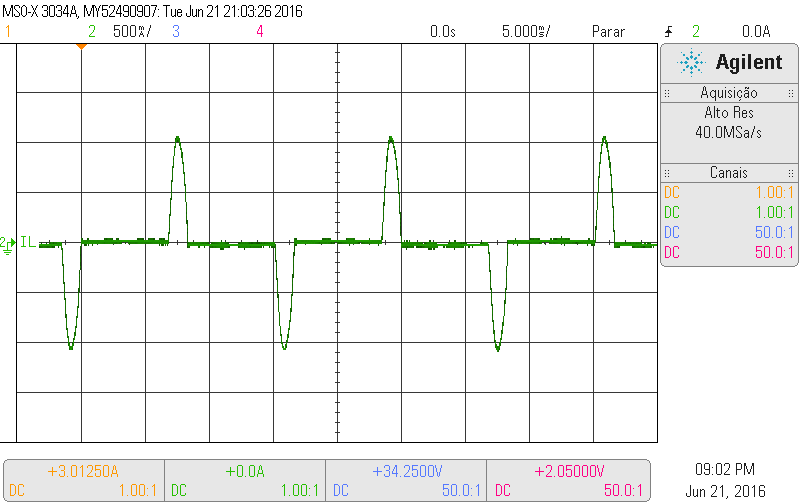
\includegraphics[width=\linewidth, center]{images/acq/scope4}
			\end{subfigure}
			\hspace*{0.02\linewidth}
			\begin{subfigure}{0.47\linewidth}
				\caption{}
				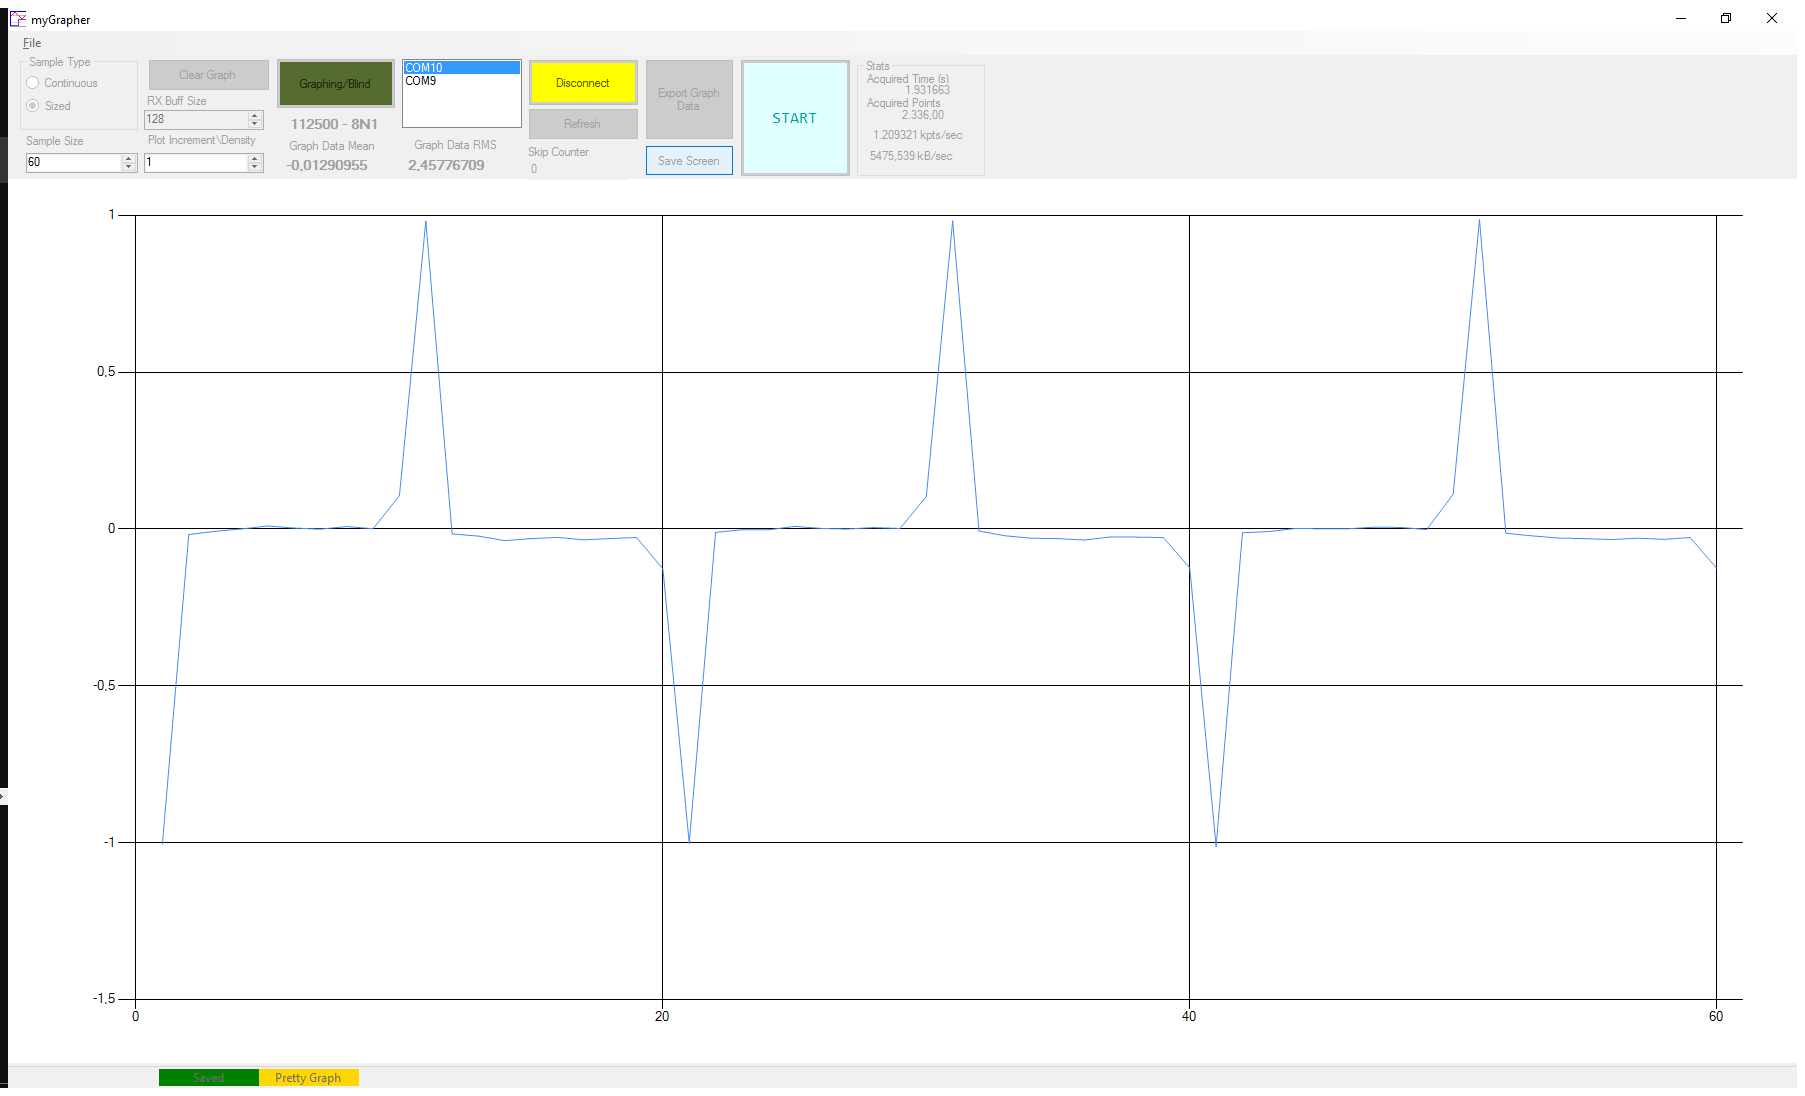
\includegraphics[width=\linewidth, clip, trim={7pt, 0cm, 0cm, 0cm}, center]{images/acq/dpo2014operation}
			\end{subfigure}
		\end{figure}

		\begin{figure}
			\caption{Corrente de alimentação CA para Fonte Tektronix\textsuperscript{\textregistered} PWS4305, (a) e (b) sem carga, (c) e (d) fornecendo 27 W}
			\label{img:proto:resul:tek}
			\centering
			\begin{subfigure}{0.47\linewidth}
				\caption{}
				\label{img:proto:resul:tekop}
				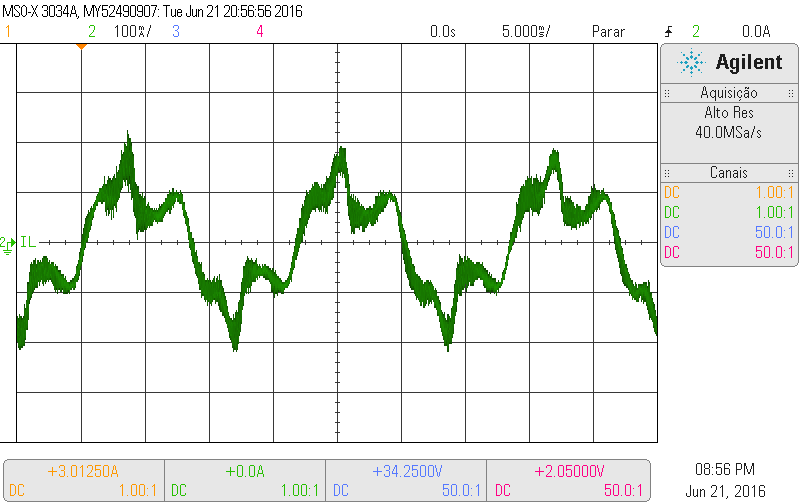
\includegraphics[width=\linewidth, center]{images/acq/scope0}
			\end{subfigure}
			\hspace*{0.02\linewidth}
			\begin{subfigure}{0.47\linewidth}
				\caption{}
				\label{img:proto:resul:tek1}
				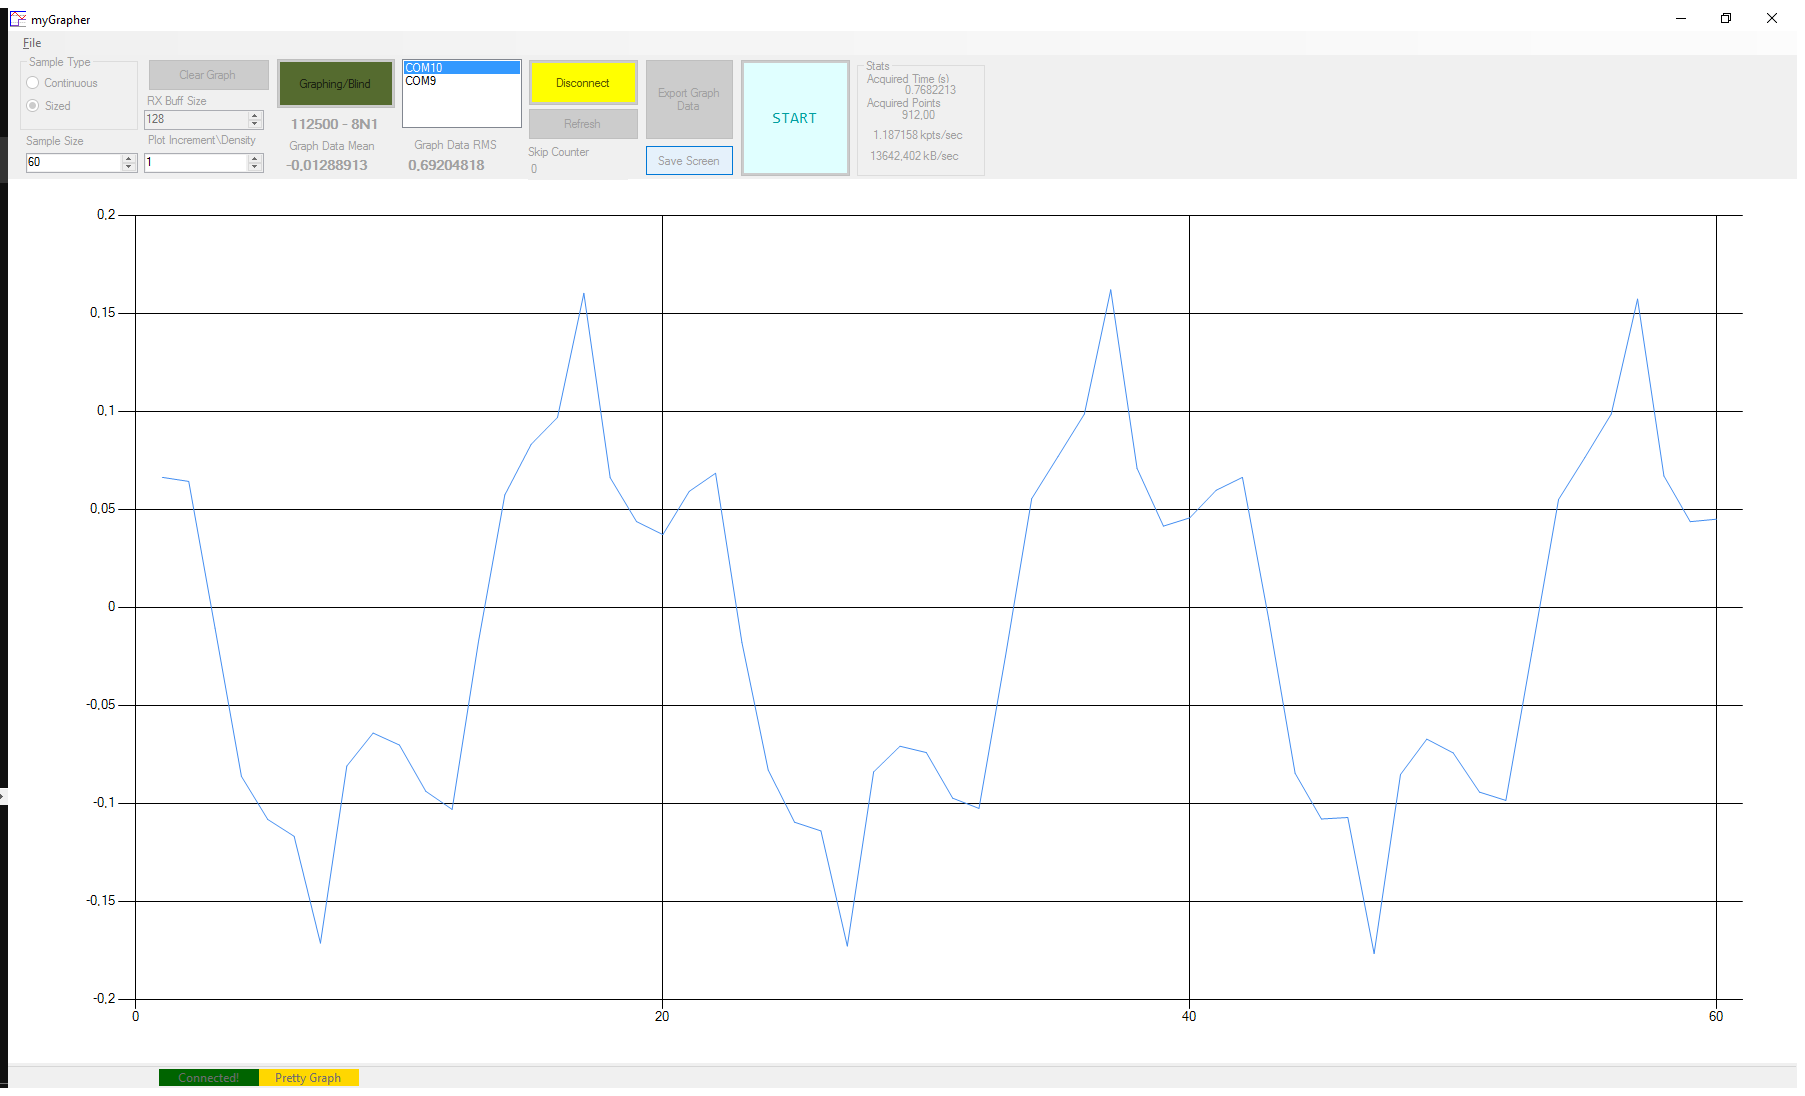
\includegraphics[width=\linewidth, clip, trim={7pt, 0cm, 0cm, 0cm}, center]{images/acq/noload}
			\end{subfigure}

			\begin{subfigure}{0.47\linewidth}
				\caption{}
				\label{img:proto:resul:tek2}
				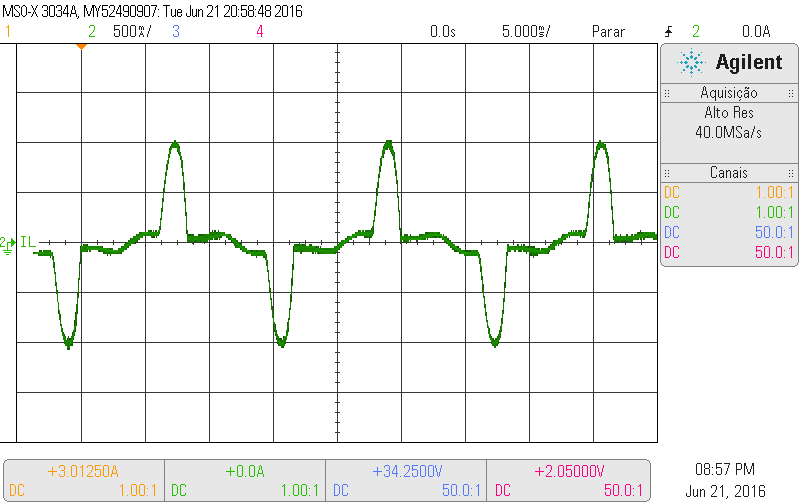
\includegraphics[width=\linewidth, center]{images/acq/scope2}
			\end{subfigure}
			\hspace*{0.02\linewidth}
			\begin{subfigure}{0.47\linewidth}
				\caption{}
				\label{img:proto:resul:tek3}
				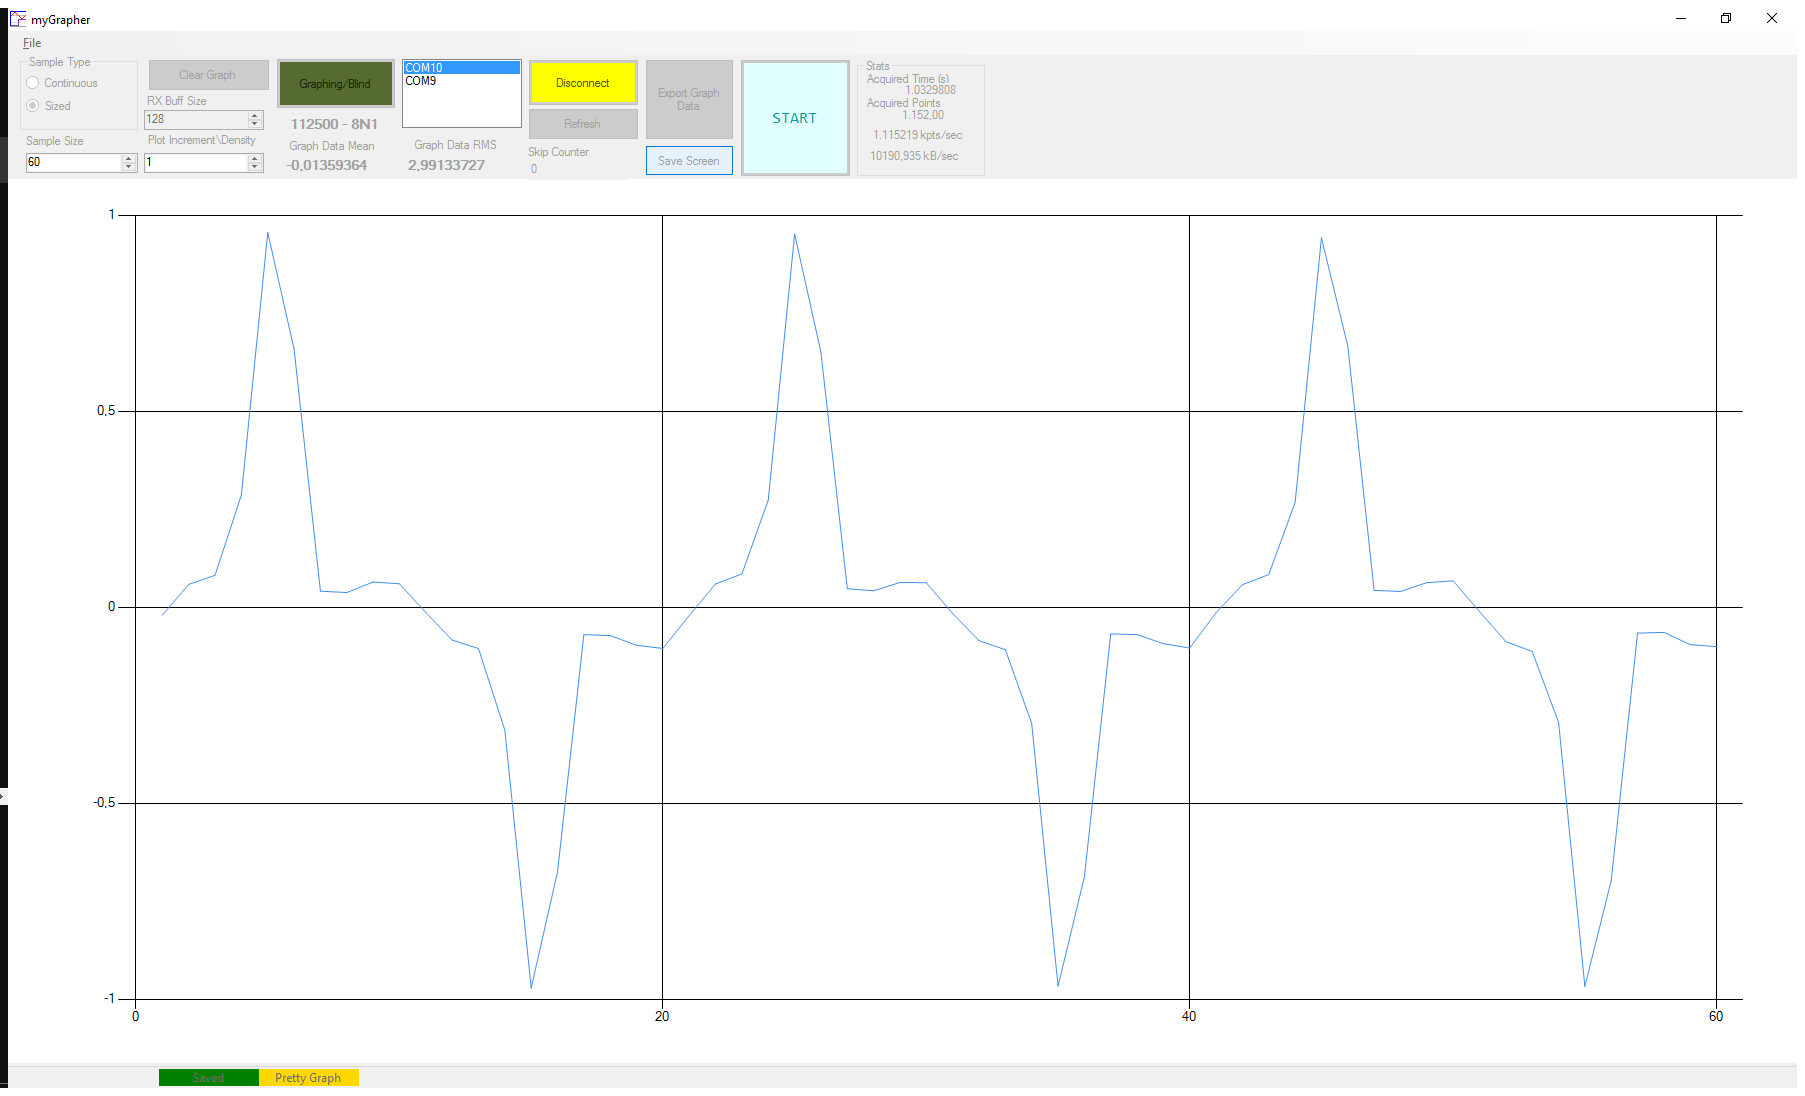
\includegraphics[width=\linewidth, clip, trim={7pt, 0cm, 0cm, 0cm}, center]{images/acq/realoneamp}
			\end{subfigure}
		\end{figure}

		\begin{figure}
			\caption{Corrente de alimentação CA para TV Samsung\textsuperscript{\textregistered} LN46B550K1V}
			\label{img:proto:result:tv}
			\centering
			\begin{subfigure}{0.47\linewidth}
				\caption{Processo de inicio de operação}
				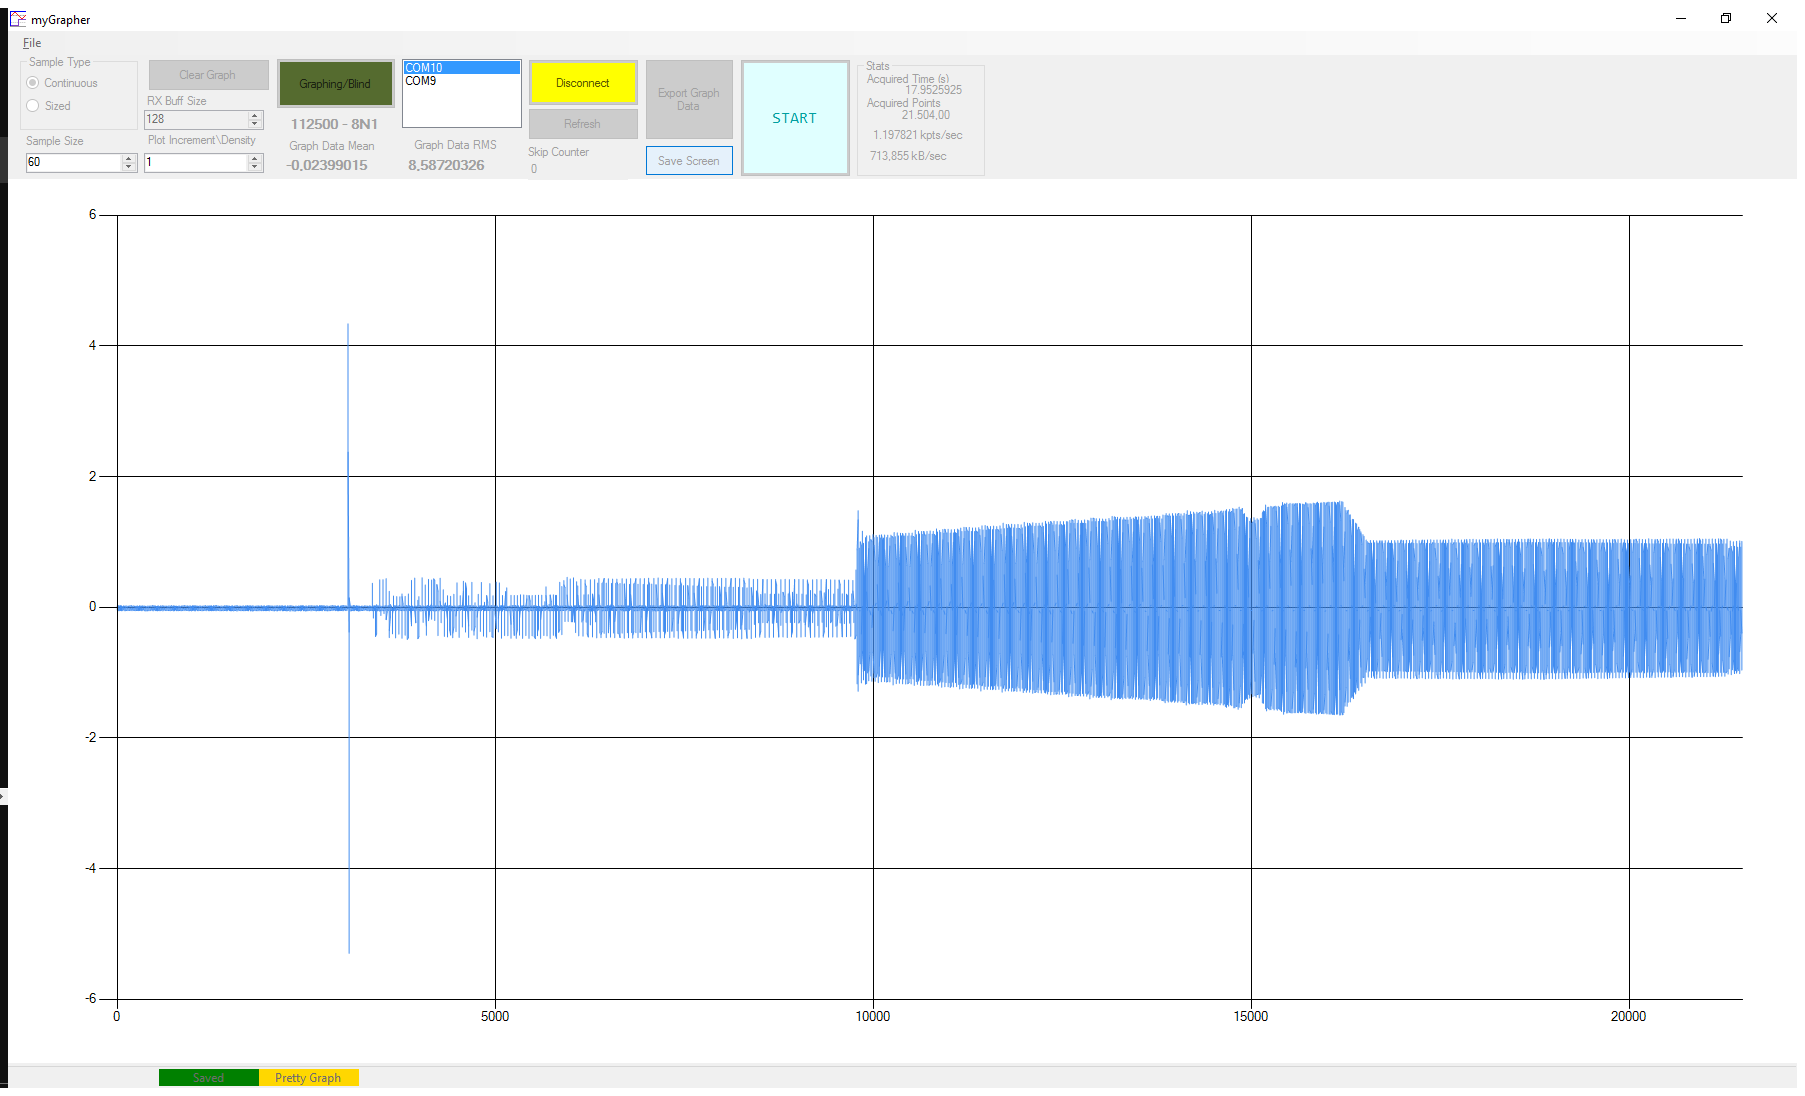
\includegraphics[width=\linewidth, clip, trim={7pt, 0cm, 0cm, 0cm}, center]{images/acq/tvcurrenturnon}
			\end{subfigure}
			\hspace*{0.02\linewidth}
			\begin{subfigure}{0.47\linewidth}
				\caption{Durante operação}
				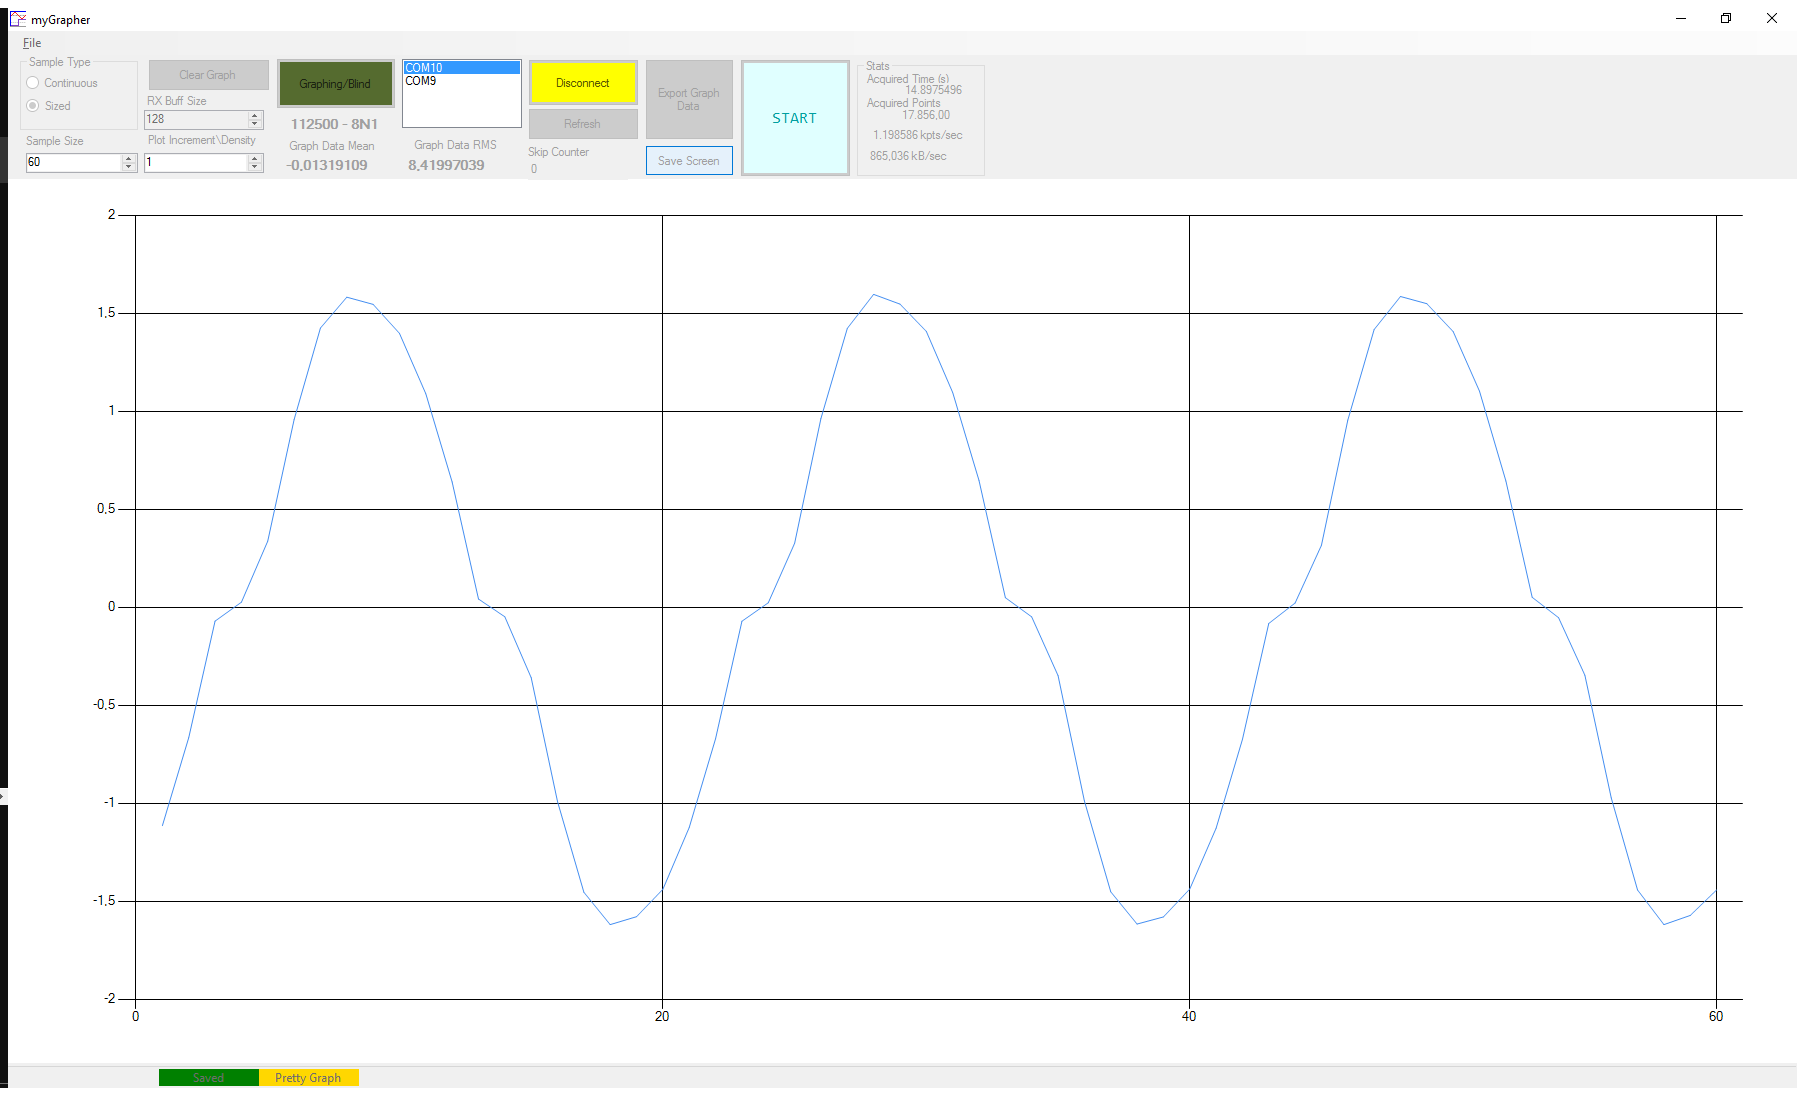
\includegraphics[width=\linewidth, clip, trim={7pt, 0cm, 0cm, 0cm}, center]{images/acq/tvcurrentop}
			\end{subfigure}
		\end{figure}

		A Figura \ref{img:proto:result:power} apresenta formas de onda para a potência durante operação da TV Samsung\textsuperscript{\textregistered} e do carregador de \textit{notebook} Sony\textsuperscript{\textregistered}. A potência apresenta espelhamento em relação ao eixo $x$ devido à conexão invertida de algum dos elementos do circuito da Figura \ref{img:proto:meas}.

		\begin{figure}
			\caption{Potência durante operação}
			\label{img:proto:result:power}
			\centering
			\begin{subfigure}{0.47\linewidth}
				\caption{TV Samsung\textsuperscript{\textregistered} LN46B550K1V}
				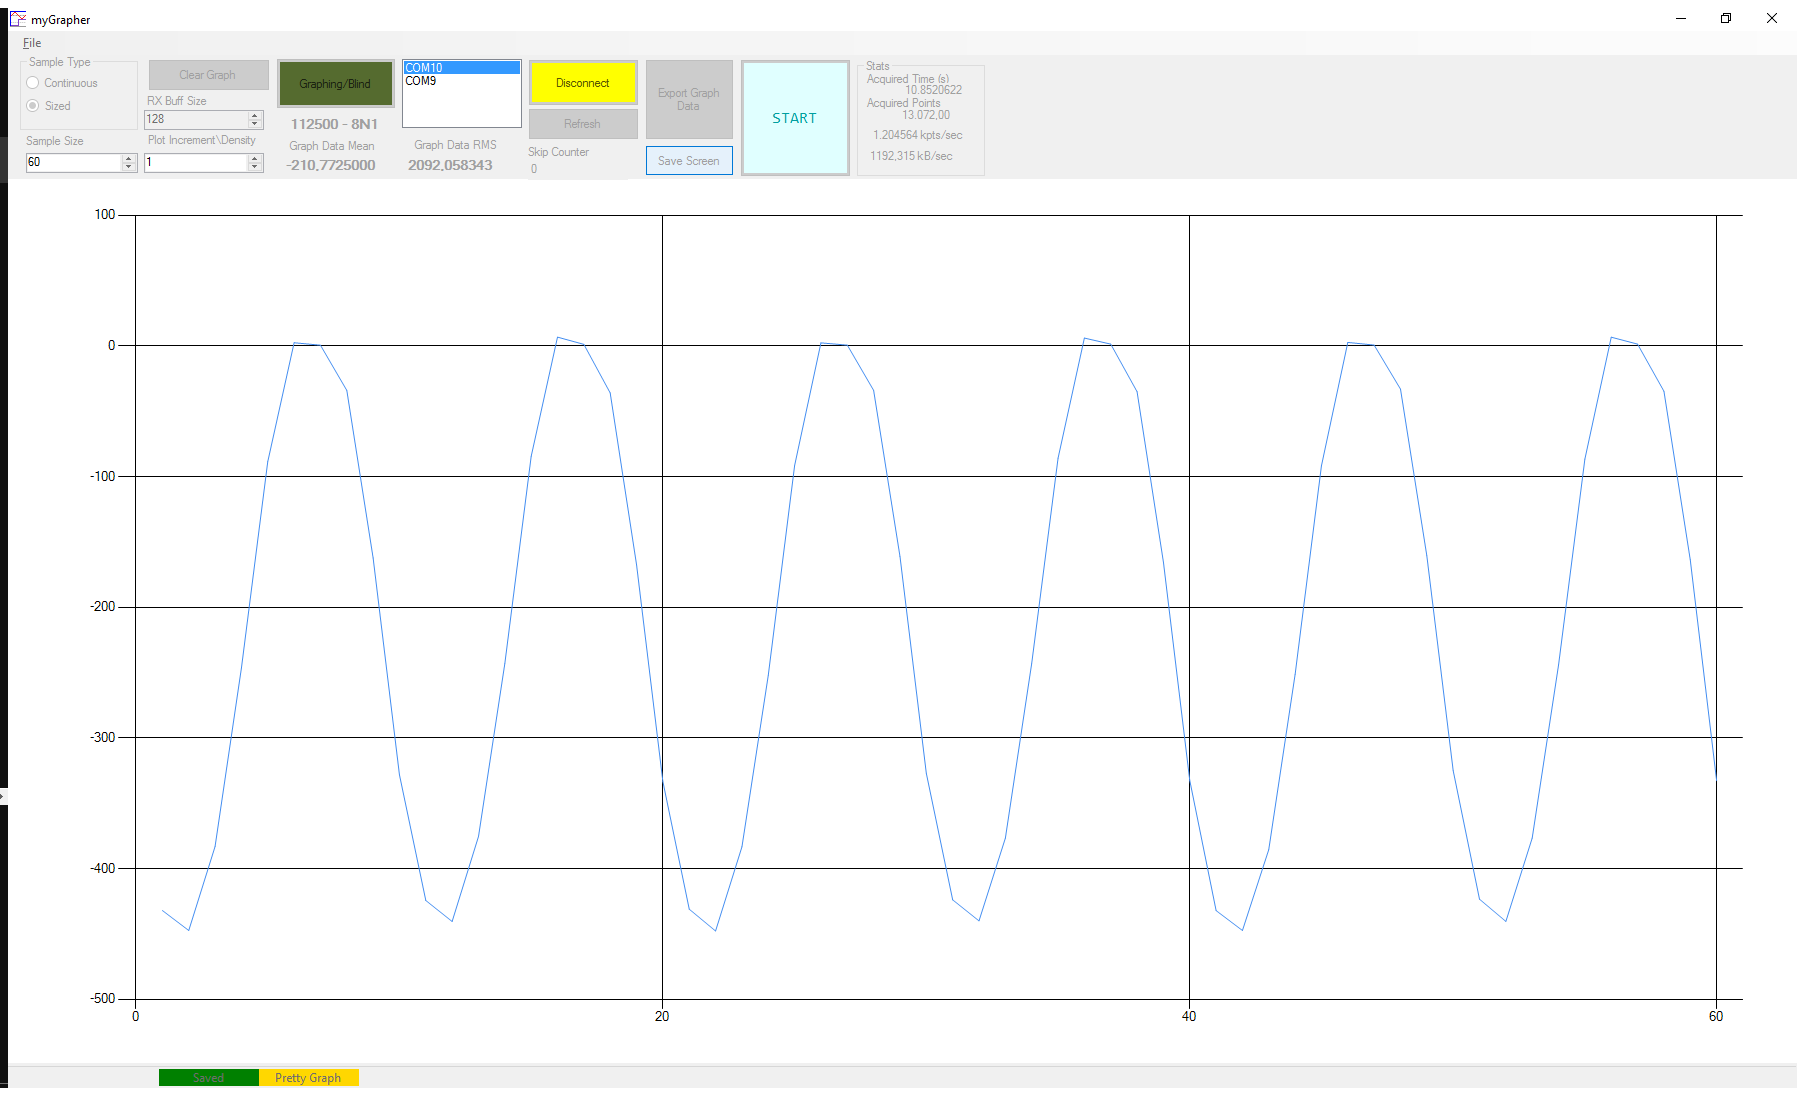
\includegraphics[width=\linewidth, clip, trim={7pt, 0cm, 0cm, 0cm}, center]{images/acq/tvpowerop}
			\end{subfigure}
			\hspace*{0.02\linewidth}
			\begin{subfigure}{0.47\linewidth}
				\caption{Carregador de \textit{notebook} Sony\textsuperscript{\textregistered} ADP-45CE}
				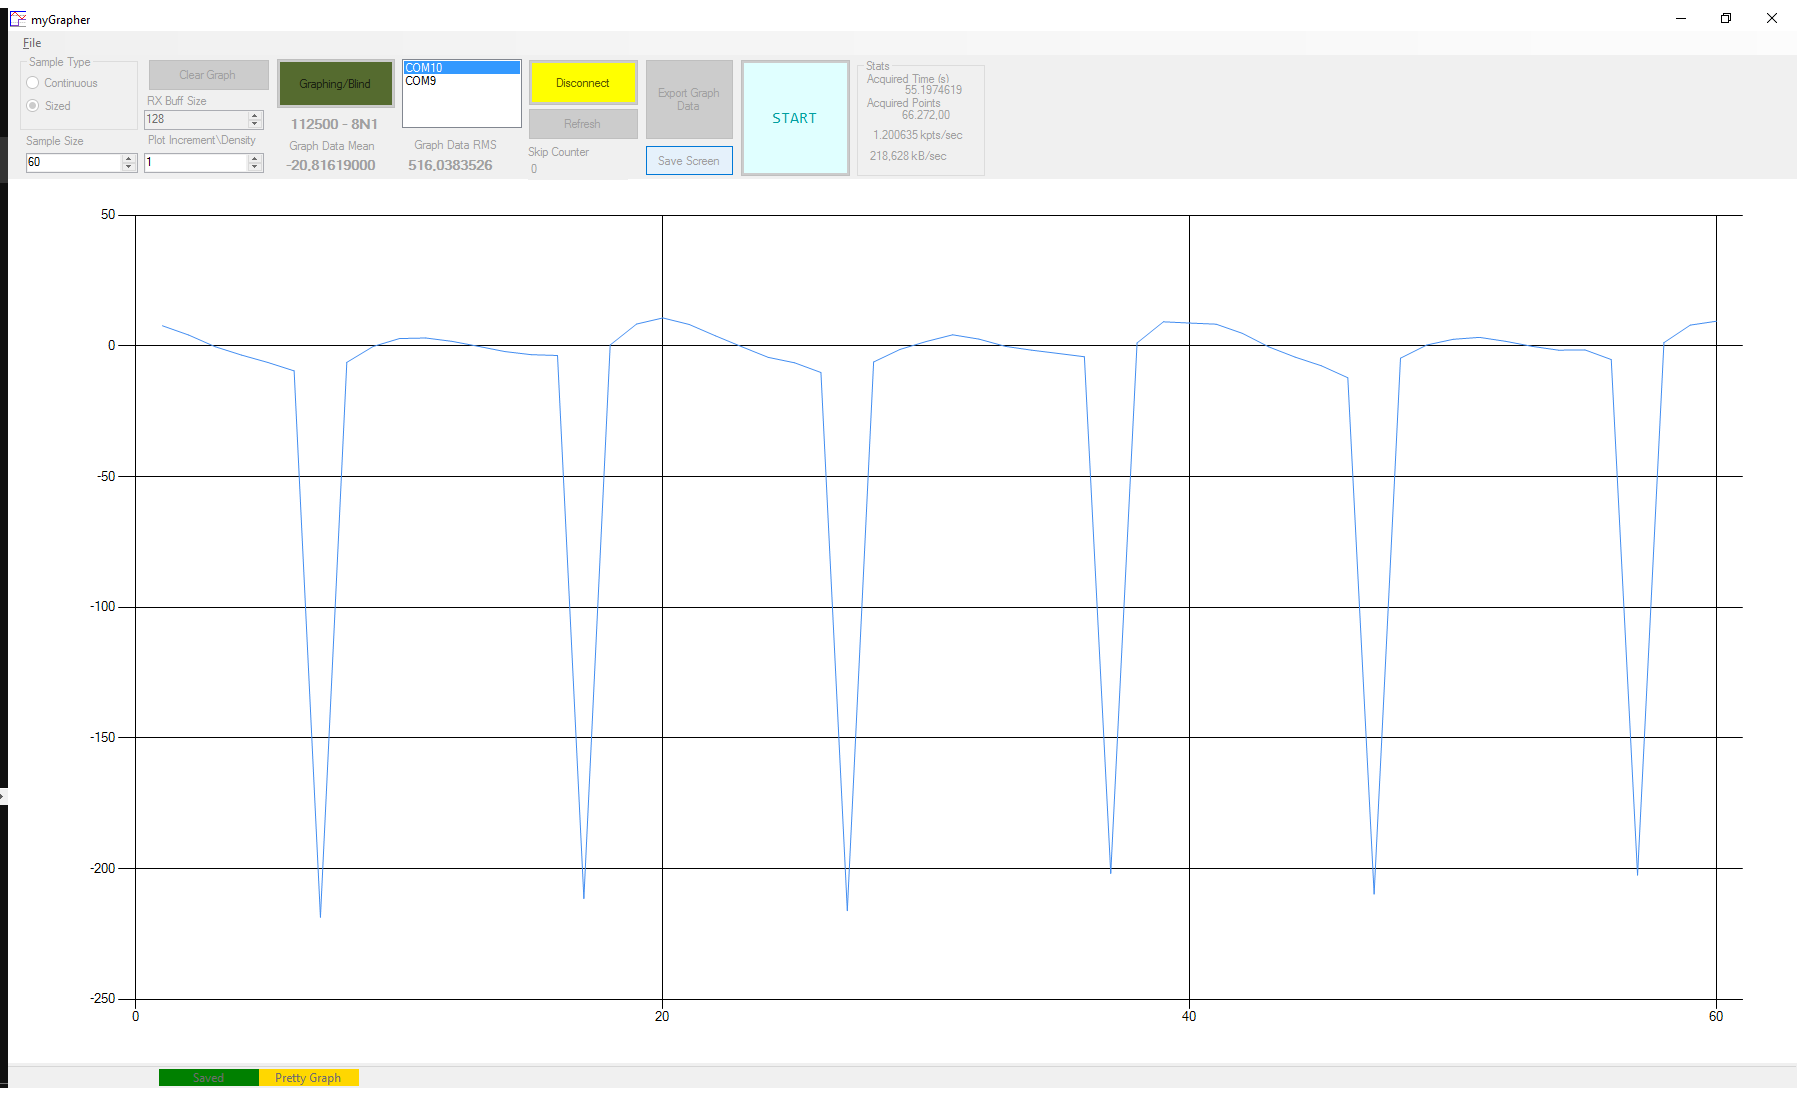
\includegraphics[width=\linewidth, clip, trim={7pt, 0cm, 0cm, 0cm}, center]{images/acq/nbpowerop}
			\end{subfigure}
		\end{figure}

		As Figuras \ref{img:proto:resul:tek} e \ref{img:proto:resul:osc} apresentam, na esquerda, imagens capturadas com um osciloscópio Agilent\textsuperscript{\textregistered} MSO-X 3034A e sonda de corrente Tektronix\textsuperscript{\textregistered} TCP312 com amplificador Tektronix\textsuperscript{\textregistered} TCPA 300. Na direita imagens capturadas com o programa \textit{myGrapher}. As Figuras \ref{img:proto:result:tv} e \ref{img:proto:result:power} foram capturadas com o programa \textit{myGrapher}.
		\index{Tektronix\textsuperscript{\textregistered}}
		\index{Agilent\textsuperscript{\textregistered}}
		\index{Samsung\textsuperscript{\textregistered}}
		\index{\textit{myGrapher}}


%you are not defending anything. stop that bitching about it. (viva)
